\subsection{Implementation Details}

The neural network model employed is a Multi-Layer Perceptron (MLP) designed to predict the quality of point clouds based on their extracted features. The architecture comprises an input layer, four hidden layers, and an output layer. Specifically, the hidden layers contain 64, 128, 128, and 64 units, respectively, and employ the ReLU activation function to introduce non-linearity. The output layer consists of a single unit that produces the final prediction value.

The model is implemented using the FLAX NNX framework, which is part of the JAX ecosystem. This enables efficient automatic differentiation and GPU acceleration, significantly reducing training times. The network is trained using the Adam optimizer, with a learning rate of 0.001 and a large batch size of 200{,}000. Training is performed for 1{,}000 epochs, and the loss function used is the mean squared error (MSE) between the predicted values and the ground truth labels.

Prior to being fed into the model, all features are standardized to improve convergence and generalization. The dataset is split into 80\% for training and 20\% for validation, ensuring that the model is evaluated on unseen data and can generalize effectively.

\begin{table}[htbp]
\centering
\begin{tabular}{|l|c|c|}
\hline
\textbf{Score} & \textbf{Dataset 1} & \textbf{Dataset 2} \\
\hline
R\textsuperscript{2} & 0.9818 & 0.9910 \\
MAE & 0.0425 & 0.0318 \\
MSE & 0.0137 & 0.0068 \\
RMSE & 0.1170 & 0.0825 \\
Max error & 1.8672 & 1.6806 \\
\hline
\end{tabular}
\vspace{0.5em}  % Adjust as needed
\caption{Comparison of model evaluation metrics between models trained on different datasets.}
\label{tab:model_metrics}
\end{table}

It is of interest to examine whether the model's predictions of surface density rely too heavily on a small subset of features. This is evaluated by analyzing which features are most influential and their relative importance in determining accurate predictions.

\begin{figure}[htbp]
\centering
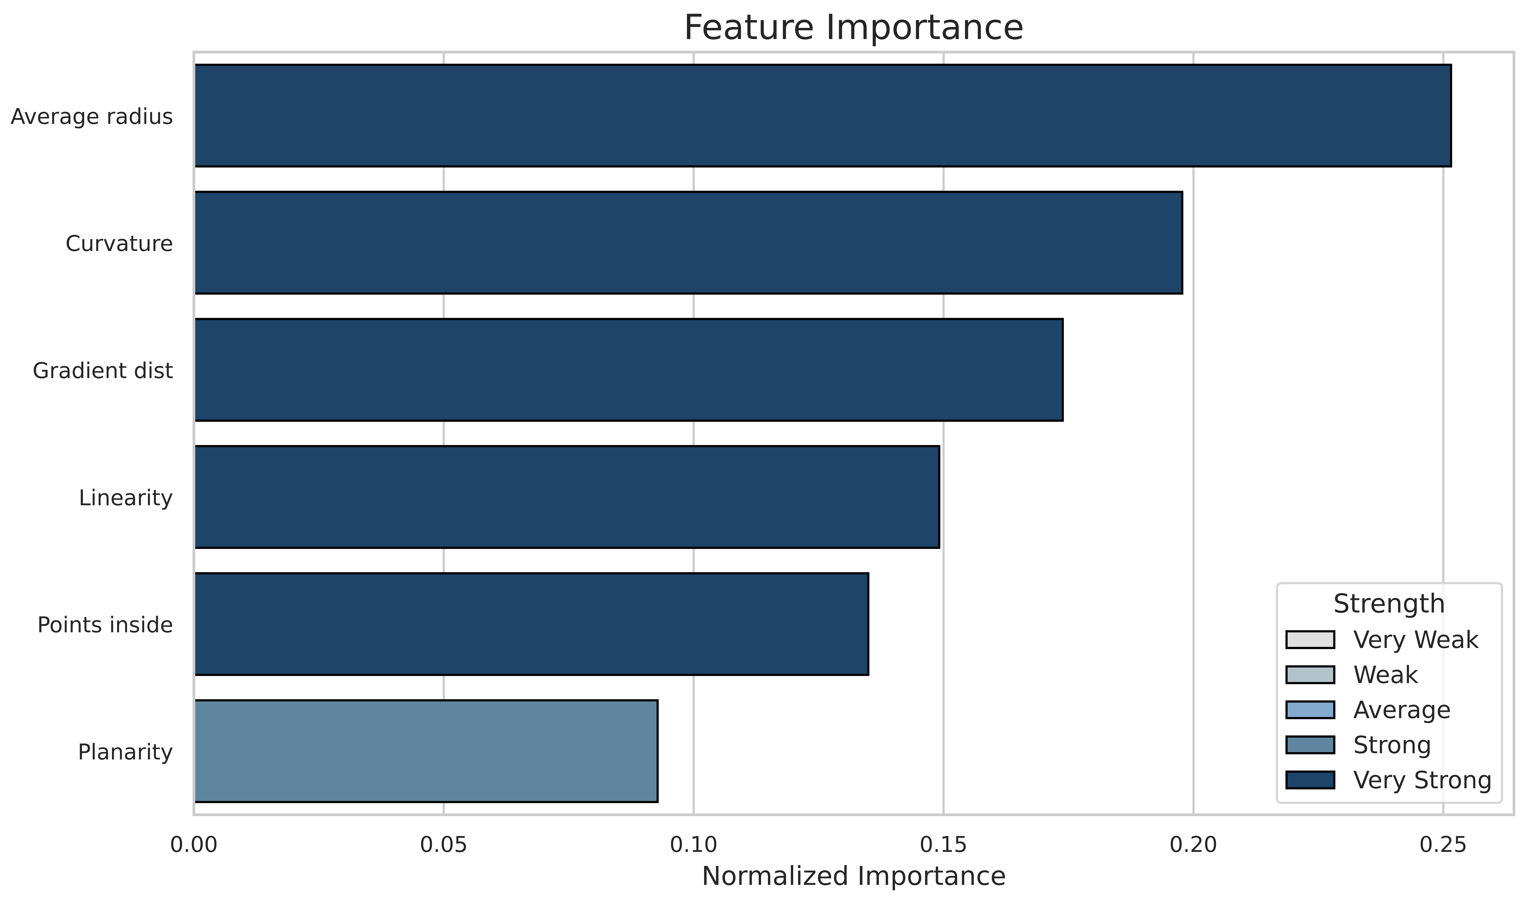
\includegraphics[width=0.5\textwidth]{figures/feature_importance_lowQ.png}
\caption{Visualization of the features used for training and their relative importance in the final model.}
\label{fig:feature_importance}
\end{figure}

A good distribution of importance between features show that the model use all features and not relying too much on a small number of features, see figure(\ref{fig:feature_importance})

While there is not a big difference in standard evaluation metrics between models trained on the two different datasets, there is a big difference the predictions of the models, especially in the lower end of mesh sizes. Therefore we need more evaluation criteria than the standard evaluation metrics.

